\chapter{Conclusions and outlook}
\label{chap:conclusions}
In this thesis analyses of proton-proton collisions recorded by the \ac{CMS} detector during
Run 1 and Run 2 of the \ac{LHC} have been presented. The focus of these analyses
is the search for \ac{BSM} Higgs bosons with tau leptons in the final state.

The search for a heavy Higgs boson decaying to a final state of $bb\Pgt\Pgt$ via two
125 GeV Higgs bosons was performed using 19.7 fb$^{-1}$ of data collected at a
centre of mass energy of 8 TeV during the 2012 \ac{LHC} data-taking period. Such a final
state can access areas of the MSSM phase space not easily accessible via other channels.
To separate more signal-like and more background-like events, a categorisation based on the number of 
b-tagged jets is used. To further increase the sensitivity to the signal, cuts on the di-tau and di-b
mass in a window around 125 GeV are used in combination with a kinematic fitting technique for
the reconstruction of the 4-body mass.
The resulting mass variable provides good separation between the signal and the dominant
\ttbar background, and is thus used as the variable for signal extraction. 
The results of this search are upper limits on production cross section times branching 
ratio, in a mass range $260<m_H<350$ GeV. A combination with a search for \AtoZhtolltautau
yields exclusion in the lowest \tanb~region of the low-tanb~MSSM scenario, as well
as several areas of the \cosba-\tanb~plane in a \ac{2HDM} scenario.

Searches for a heavy neutral Higgs boson decaying into pairs of tau leptons were performed
using 2.3 fb$^{-1}$ of data recorded during the 2015
data-taking period of the \ac{LHC}, and using 12.9 fb$^{-1}$ of 
data recorded during the first half of the 2016 data-taking period. The 
branching ratio of heavy neutral Higgs bosons into di-\Pgt pairs is enhanced at high \tanb~in the \ac{MSSM},
making this one of the most sensitive search channels for such particles. The analysis uses a categorisation 
based on the presence of b-tagged jets to separate
the gluon fusion and b-associated production modes of Higgs bosons in the \ac{MSSM}. 
The hadronic tau isolation working point, as well as the topological selection on 
the \mT~variable, are chosen to optimise the search sensitivity for signal
masses of around 1 TeV.
The sensitivity is maximised by using the \mTtot~variable for signal extraction.
This variable separates the dominant backgrounds
and the high-mass signal well.
No significant excess is observed in these searches, and so 
these analyses set limits on the production cross section times branching ratio of both the
gluon fusion and b-associated production processes. The results are also
interpreted in MSSM benchmark scenarios, where the analyses exclude large areas
of the \mA-\tanb~plane, with significant improvement with respect to the most sensitive
results obtained in Run 1. A combination of the 2015 and 2016 analyses is also
performed. This combination improves on the results of the 2016 analysis alone, thus
setting the most stringent limits on this process to date.

As more data are collected during the remainder of Run 2, and in the 
future, searches for MSSM Higgs bosons in the di-$\Pgt$ final
state will continue. If no such Higgs bosons are found, these searches
will be able to exclude even more of the \mA-\tanb~plane in specific
MSSM benchmark scenarios, although not all of the \mA-\tanb~plane
will become accessible. A projection of the results of the 2015 \ac{MSSM}
analysis to an integrated luminosity of 300 fb$^{-1}$ and 3000 fb$^{-1}$ is
shown in figure \ref{fig:mssm_projection_fig}. Even with an integrated luminosity of
3000 fb$^{-1}$ it is not possible to exclude the full \mA-\tanb~plane of this scenario,
as the branching ratio of $\PHiggsps/\PHiggs$ into di-$\Pgt$ pairs 
is very low in the high \mA-low \tanb~corner. This region can be accessed 
via searches for the $\PHiggsps/\PHiggs \rightarrow \Ptop\APtop$ decay, which
has an enhanced branching ratio in this region. To fully cover the still
available phase space it will therefore start to become more and more
important to combine searches for heavy Higgs bosons in different final states.
Doing this will give the best sensitivity to possible
heavy Higgs bosons - or in the absence of these particles exclusion
of the scenarios that predict them.

\begin{figure}[h!]
\begin{center}
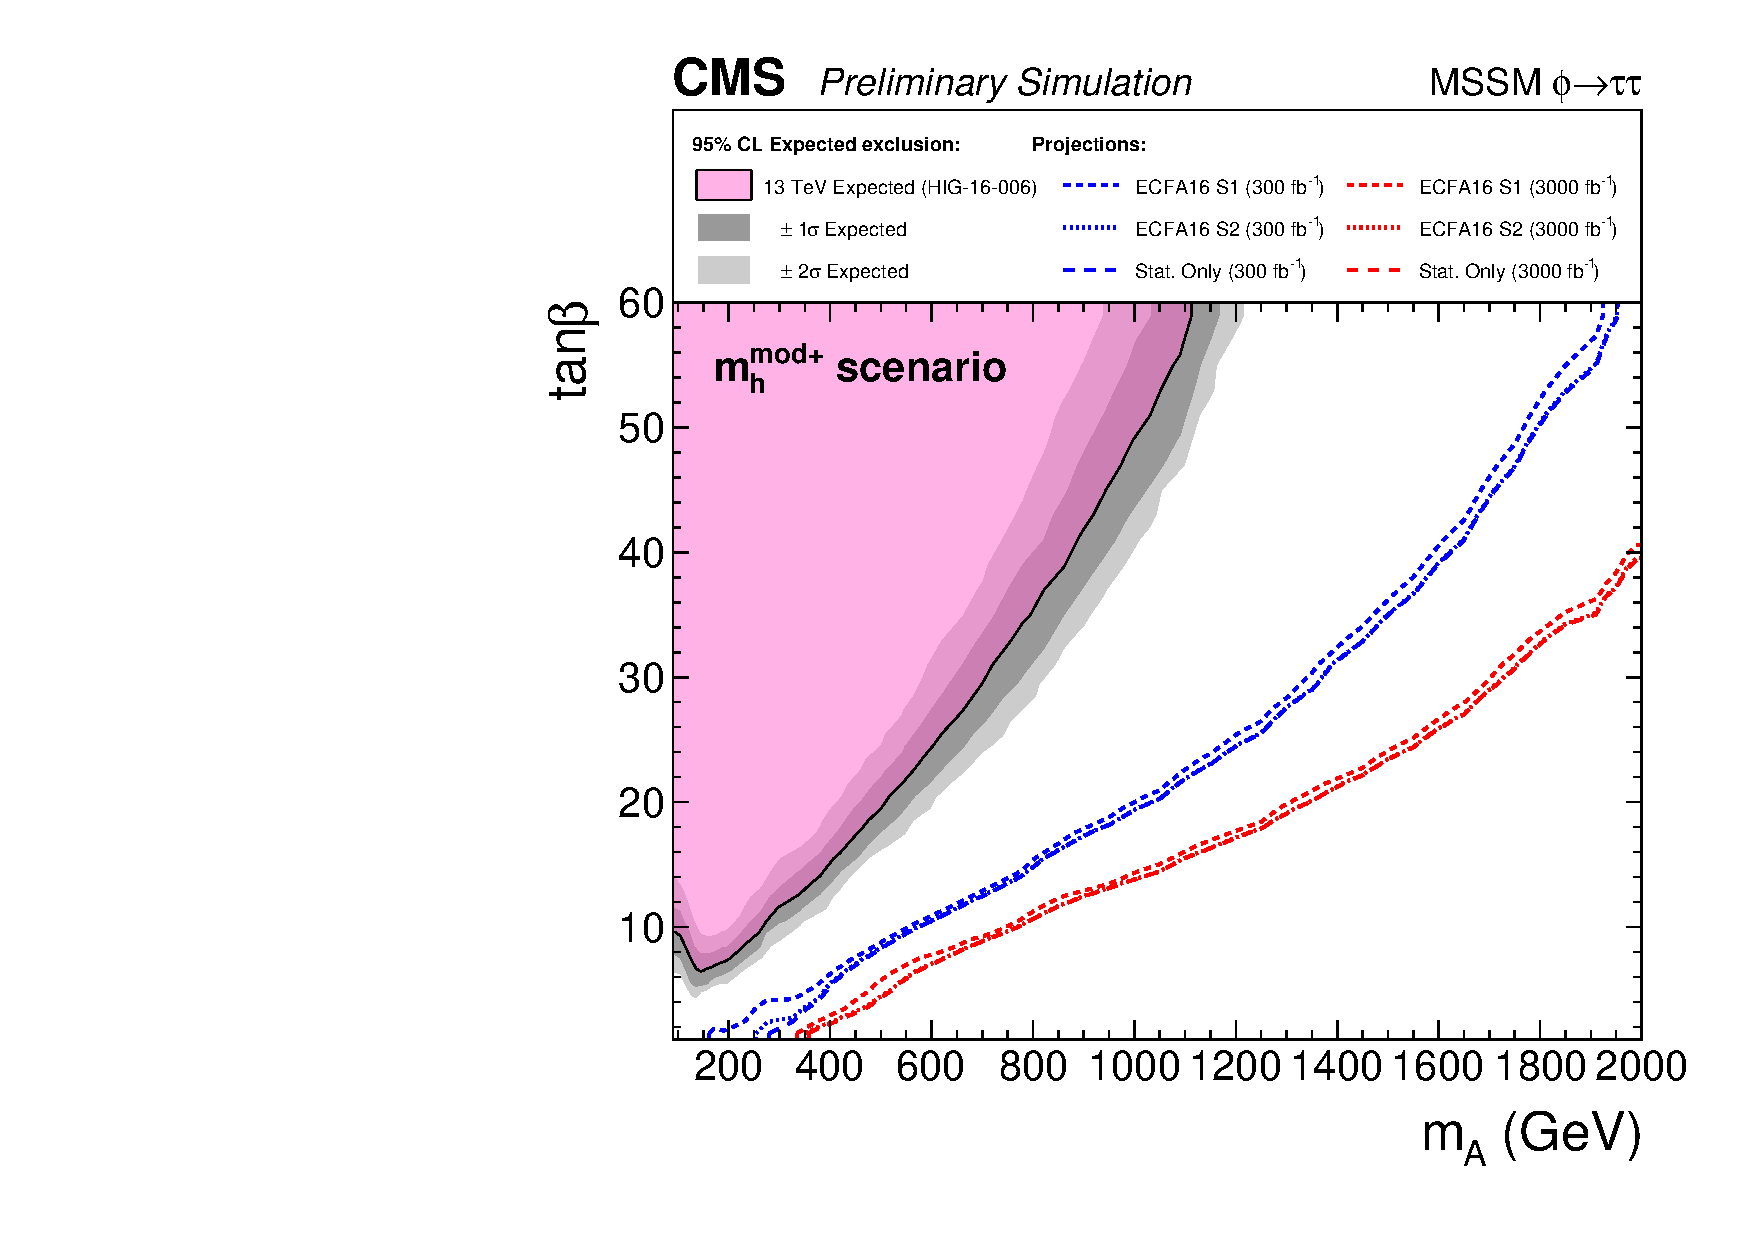
\includegraphics[width=0.7\textwidth]{./Conclusion/Figures/scenario_comp2.pdf}
\end{center}
\caption[The expected exclusion in the $m_{h}^{\text{mod+}}$ scenario
at 95\% CL of the 2015 MSSM analysis, projected to an integrated luminosity of 300-3000 fb$^{-1}$.]{The expected exclusion in the $m_{h}^{\text{mod+}}$ scenario
 at 95\% CL of the 2015 MSSM analysis (pink)
projected to an integrated luminosity of 300 fb$^{-1}$ (blue) and 3000 fb$^{-1}$ (red)
under several assumptions of how the systematic uncertainties scale. Even with an integrated 
luminosity of 3000 fb$^{-1}$ it is not possible to exclude the entire \mA-\tanb~plane
in this \ac{MSSM} benchmark scenario \cite{HTT-projection}.}
\label{fig:mssm_projection_fig}
\end{figure}

